% ------------------------------------------------------------------- %
% ------------------------------------------------------------------- %
\chapter{Overview}
\label{sec:overview}

The goal of this chapter is to give an as brief but complete overview of the theoretical and algorithmic pieces needed to understand the inputs for, and outputs of the MORIS mesh generation.
%This chapter will lay out the some pieces of theory that are beneficial to understanding the mesh generation and its output. 
As mentioned in the foreword, the output data is intended to perform interpolation-based immersed finite element analysis, the theory for which, with the exception of a brief introduction to \hyperref[sec:overview_extraction]{Lagrange extraction}, will not be discussed in this document. Instead the reader is advised to consult the publication by Fromm et al. \cite{Fromm2022}

\refpar{moris_overview}{MORIS} ("Multi-physics Optimization Research and Innovation System") is a standalone finite element and topology optimization software framework. The analysis method utilized inside of MORIS itself is a quadrature-based immersed isogeometric method. The interpolation function basis is provided by a rectangular tensor-product B-spline mesh, the \textbf{background mesh}, that can be hierarchically refined. Next, geometries are immersed into said mesh. The geometry is described implicitly by level-set fields $\Phi(\bm{x})$ and their iso-contours  $\Phi(\bm{x}) = c$. A quadrature rule for evaluating the discretized weak form is found by tessellating, or \hyperlink{decomposition}{"\emph{decomposing}"}, the background mesh's elements intersected by the iso-contours into triangles or tetrahedrons whose Gauss points and weights provide the integration rule. Additionally, the background basis is heaviside enriched to solve problems with multiple materials. For the interested reader, the isogeometric analysis framework inside of MORIS is explained in more detail in Schmidt et al. \cite{Schmidt2022}.

The set of non-intersected background elements and triangular elements within intersected elements together form a body-fitted mesh which from here on will be referred to as the \textbf{foreground mesh}. This body-fitted foreground mesh and its known relation to the background mesh it is constructed from together form the mesh information needed for interpolation-based immersed analysis. Hence, the mesh generation abilities of MORIS can directly be exploited to provide all mesh information needed to also perform interpolation-based immersed finite element analysis.

The meshing apparatus inside MORIS consists of three modules: a hierarchical B-spline mesh generator called HMR, a geometry engine (GEN), and an extended finite element tool kit (XTK). To obtain the desired meshes, the inputs for these three modules need to be configured. More specifically, HMR needs to be fed what the size, dimensions, and order of its tensor-product meshes is, and how they're to be refined. GEN needs level-set fields to determine interface locations and material membership. XTK works based off the information by the other modules, apart from minor configuration input. A \hyperref[fig:workflow]{chart of the workflow} is shown below.

\begin{figure}[h]
    \vspace{0.5cm}
    \begin{center}
    %\def\svgwidth{15.0cm}
    \input{Figures/workflow.pdf_tex}
    \caption{Workflow for mesh generation inside MORIS} 
    \label{fig:workflow}
    \end{center}
\end{figure}

The remainder of this chapter is laid out as follows. First, a short introduction on how \hyperref[sec:overview_geometry]{geometries} can be defined with level-set fields will be given. Next, the \hyperref[sec:overview_background]{interpolation basis} used by MORIS is defined alongside the enrichment strategy used. Lastly, the \hyperlink{decomposition}{algorithm for generating the foreground mesh} is shown and how the \hyperref[sec:overview_extraction]{extraction operators} are computed from it.

\paragraph{Note:} The features currently supported in the pure mesh generation workflow do not include all features supported by MORIS internally, but are undergoing expansion to do so. Until then, some parts of this chapter may seem unnecessary. 

% \hyperref[sec:overview_workflow]{workflow}
% \hyperlink[enrichment]{enrichment}

% ------------------------------------------------------------------- %
\section{Geometry}
\label{sec:overview_geometry}

As mentioned above, geometry in MORIS is described implicitly by a level-set field $\Phi_i(\bm{x})$ and a threshold $c$, which is assumed to be $c=0$ from here on, determining the locations of interfaces. 
This leads to a straight forward definition of what is \emph{inside} and \emph{outside} of a given geometry. 

\begin{equation}
\label{eq:level_set_field}
    \Phi_i(\bm{x}) 
    \begin{cases}
        < 0 & \bm{x} \notin \Omega_i \\
        = 0 & \bm{x} \in \partial\Omega_i \\
        > 0 & \bm{x} \in \Omega_i \\
    \end{cases}
\end{equation}

\hypertarget{phase_assignment}{}
If multiple level-set fields, and therefore geometries, are introduced, each point $\bm{x}$ is defined to be either inside or outside with respect to each of the geometries. Each region of points that is a certain combination inside/outside with respect to each of the geometries is called a \emph{phase}. This leads to there being up to $n_p = 2^{n_{LSF}}$ phases inside a given domain, when $n_{LSF}$ geometries are defined. \emph{Material} sub-domains can simply be defined by merging these phases, as illustrated in \Cref{fig:phase_mergin}

\begin{figure}[h]
    \begin{center}
    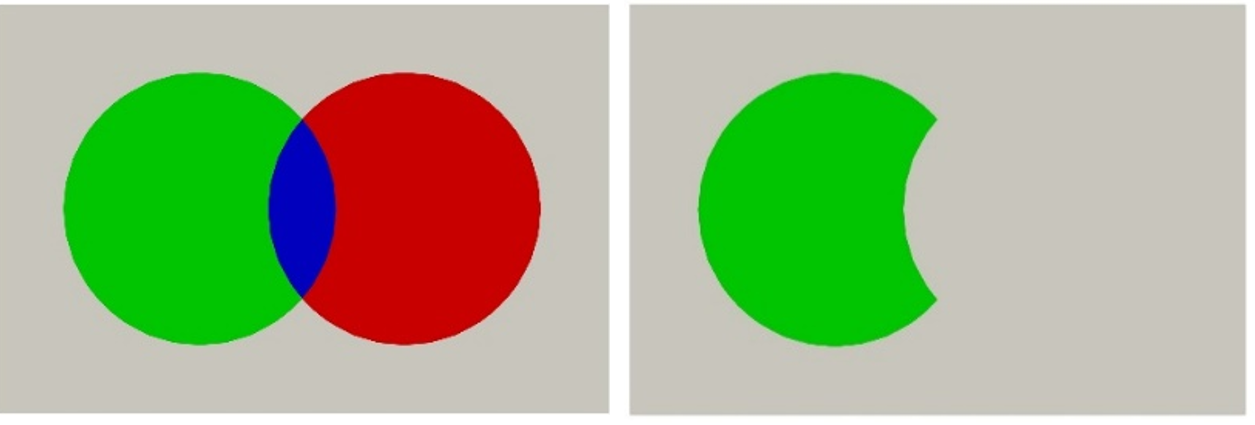
\includegraphics[width=10cm]{Figures/phase_merging.png}
    \caption{Introducing two discs as geometries into an ambient domain results in four phases (marked in different colors). Material domains can be defined by merging phases. } 
    \label{fig:phase_mergin}
    \end{center}
\end{figure}

A particularly notable type of level-set field is a so-called signed-distance field, which is a field at which every point has a value whose magnitude corresponds to the minimum distance to an interface.
Any geometry definition that has a notion of "inside" and "outside" can be converted to a signed-distance field and therefore be used with MORIS (if a pre-processor for the conversion exists).

% ------------------------------------------------------------------- %
\section{Background Basis and Enrichment}
\label{sec:overview_background}

TODO...

% ------------------------------------------------------------------- %
\section{Foreground Mesh}
\label{sec:overview_foreground}

As mentioned in the \hyperlink{moris_overview}{overview of MORIS}, the foreground mesh is generated by decomposing the background mesh, or more precisely one of the background grids. This process will be referred to as the \emph{decomposition}.

\refpar{decomposition}{The Decomposition} consists of three steps which are also visualized in \Cref{fig:decomposition}
\begin{itemize}
    \item The first step is to identify which particular background elements are intersected and need to be decomposed. To do so, the values of all level-set fields $\Phi_i(\bm{x})$ is checked at the vertices, i.e. the "corners", of the background element. If a sign change is detected between level-set values, the element is marked for decomposition. Note, that due to this particular way of intersection detection, elements that may contain material enclosures that are completely contained within itself, or protrude that background element on only one facet, may not be decomposed.

    \item \hypertarget{regular_subdivision}{In a next step,} each intersected background element is subdivided into triangles or tetrahedrons, depending on dimensionality. This step will be referred to as the \emph{regular subdivision}.

    \item The edges of the triangular elements created in the regular subdivision can again be checked for sign changes in the level-set fields. Depending on which edges of a given triangle or tetrahedron are intersected, the element can be further subdivided into a pre-defined set of triangles or tetrahedrons.
    This step is subsequently repeated for each geometry in the order that the level-set fields are defined. Hence, the resulting foreground mesh may differ slightly depending on the order in which the level-set fields are defined.

    \item All elements are assigned a material membership based on the signs of the level-set functions, as \hyperlink{phase_assignment}{discussed previously}.
    
    \item At this point the elements are just geometric entities. By placing nodes at the vertices linear elements are obtained. Higher order elements are obtained by positioning equispaced (with respect to a standardized parametric element) nodes along the edges and the inside of the resulting triangles and tetrahedrons.
\end{itemize}
A detailed discussion of this decomposition procedure can be found in Doble et al. \cite{Doble2023} 

\begin{figure}[h]
    \vspace{0.2cm}
    \begin{center}
    %\def\svgwidth{15.0cm}
    \input{Figures/decomposition.pdf_tex}
    \caption{Decomposition of a background mesh grid into a geometry-fitted foreground mesh.} 
    \label{fig:decomposition}
    \end{center}
\end{figure}

\vspace{0.5cm}

The \hyperlink{decomposition}{decomposition process} layed out above leads to a foreground mesh with the \hypertarget{foreground_mesh_properties}{properties} listed below.
\begin{itemize}
    \item The element facets created during the templated triangulation are straight. Therefore, the \textbf{approximation of the geometry is piecewise linear}.
    
    \item Since the foreground mesh constructed by decomposition of a background grid, it is \textbf{background-fitted} as defined by Fromm et al. \cite{Fromm2022}.
    
    \item Further, the \textbf{quality of the geometry approximation is influenced by the resolution of the background grid} that is decomposed. Quadtree or octree refinement around the interfaces may be performed to improve the geometry representation.
    
    \item The simple algorithmic decomposition may lead to \textbf{triangular elements of extremely poor quality} (large aspect ratios, very high maximum angles). For interpolation-based immersed analysis the poor element quality is generally not of concern though.

    \item Non-intersected quadrilateral or hexahedral background elements are not decomposed. The resulting foreground mesh therefore contains a \textbf{mix of triangular and rectangular elements}. Non-intersected elements may additionally be marked for regular subdivision, though.

    \item If a hierarchically, i.e. locally, refined background mesh grid is used for decomposition, the \textbf{foreground mesh may contain hanging nodes}, like shown in \Cref{fig:decomposition}.
\end{itemize}

% ------------------------------------------------------------------- %
\section{Lagrange Extraction}
\label{sec:overview_extraction}

Lastly, it should be useful to recap the basics of Lagrange extraction. 
The key to performing interpolation-based analysis is the fact that Lagrange basis functions $\phi_j(\bm{x})$ are \emph{interpolatory}, i.e. they are $=1$ at exactly one nodal point, and $=0$ at every other nodal point $\hat{\bm{x}}_i$. An illustration for linear Lagrange basis function inside a triangular element is provided on the right of \Cref{fig:lagrange_extraction}.

\begin{equation}
\label{eq:interpolatory}
    \phi_i(\hat{\bm{x}}_i) =
    \left\{
    \begin{array}{@{}c@{}}
        1 ~~~ j=i \\
        0 ~~~ j \neq i
    \end{array} 
    \right\} 
    = \delta_{ij}
\end{equation}
    
\begin{figure}[h]
    \vspace{0.2cm}
    \begin{center}
    %\def\svgwidth{15.0cm}
    \input{Figures/Lagrange_basis_functions.pdf_tex}
    \caption{Lagrange extraction.} 
    \label{fig:lagrange_extraction}
    \end{center}
\end{figure}

A Lagrange element can be placed into another mesh that may provide another type of interpolation $u^{h,B} = \sum_{j=1}^{n} N_j^B(\bm{x}) \cdot d_j$. The two interpolations $u^{h}$ can be assumed to be approximately equal to each other (in a mathematically crude fashion).

\begin{equation}
\label{eq:approx}
\begin{split}
    u^{h,B} 
    &\approx u^{h,L} \\
    \sum_{j=1}^{n} N_j(\bm{x}) \cdot d_j 
    &\approx \sum_{i=1}^{\nu} \phi_j(\bm{x}) \cdot c_j
\end{split}
\end{equation}

Substituting identity \eqref{eq:interpolatory} into the equation at the nodal points $\hat{\bm{x}}_i$ yields the extraction operator $M_{ij}$ relating the degrees of freedom of the two bases to each other.

\begin{equation}
    \label{eq:derive_extraction_operator}
    \begin{split}
        \sum_{j=1}^{n} N_j(\hat{\bm{x}}_i) \cdot d_j 
        &\approx \sum_{i=1}^{\nu} \phi_j(\hat{\bm{x}}_i) \cdot c_j \\
        \sum_{j=1}^{n} M_{ij} \cdot d_j 
        &\approx \sum_{i=1}^{\nu} \delta_{ij} \cdot c_j \\
        \sum_{j=1}^{n} M_{ij} \cdot d_j 
        &\approx c_i \\
    \end{split}
\end{equation}

Hence, the extraction operator can be obtained simply by evaluating the background basis functions $N_j(\bm{x})$ at the nodal points of the foreground mesh $\hat{\bm{x}}_i$.

\begin{equation}
\label{eq:extraction_operator}
    M_{ij} =  N_j(\hat{\bm{x}}_i)\\
\end{equation}

Note that due to the enrichment of the basis of the background mesh to decouple different materials, nodes positioned along an interface will have different non-zero background basis functions associated with them depending on with respect to which material equation \eqref{eq:extraction_operator} is evaluated.  

\begin{equation}
\label{eq:interpolated_basis}
    \mathcal{V}^h = span\left\{ 
        \widehat{N}_j(\bm{x}) = \sum_{i=1}^{\nu} M_{ij} \cdot \phi_i
    \right\}_{j=1}^{n}
\end{equation}

Using \eqref{eq:derive_extraction_operator}, the elemental stiffness matrices $A^{(e)}$ and force vectors $B^{(e)}$ assembled in a "standard" finite element procedure can easily be projected into the space of the background mesh, or more precisely, the \emph{interpolated} background basis \eqref{eq:interpolated_basis}.

\begin{equation}
    \label{eq:transform_elemental}
    \begin{split}
        K^{(e)} &= \sum_{j,k} M_{ji} \cdot A^{(e)}_{jk} \cdot M_{kl} \\
        F^{(e)} &= \sum_{j} M_{ji} \cdot B^{(e)}_{jk}  \\
    \end{split}
\end{equation}